\begin{cuzchapter}{使用指南}{chap:guide}

    %---------------------------------------------------------------------------%
    %->> 本平台使用指南
    %---------------------------------------------------------------------------%
    % 本章主要提供本平台的使用指南和示例，帮助用户快速上手
    % 一个完整的使用指南章节应包含以下几个部分：
    % 1. 平台概述与快速入门：介绍平台基本概念和快速开始方法
    % 2. 核心功能使用指南：详细说明实时协作、权限管理、AI辅助等核心功能的使用方法
    % 3. 高级功能详解：介绍版本控制、代码片段、空间管理等高级功能
    % 4. 最佳实践与技巧：提供使用技巧和常见问题的解决方案

    \section{平台概述与快速入门}\label{sec:overview-quickstart}

    本平台是基于现代Web技术构建的智能幻灯片协作平台，旨在为技术团队和教育工作者提供高效的幻灯片制作与协作解决方案。本章将详细介绍平台的使用方法和各项功能，帮助用户快速上手并充分利用平台的协作与创作能力。

    本平台采用前后端分离架构设计。前端使用React 19、TypeScript和Vite技术栈，集成了CodeMirror 6编辑器和Yjs协作库。后端基于NestJS框架，提供RESTful API和基于Hocuspocus的WebSocket协作服务。平台支持实时协作编辑、细粒度权限管理、AI辅助创作和简化版本控制等核心功能。

    \subsection{注册与登录}

    首次使用本平台需要进行用户注册和登录：\textbf{注册账号}：访问平台网址，点击注册按钮，输入邮箱地址、用户名和密码完成注册。平台采用注册码机制，需要有效的注册码才能完成注册流程。\textbf{登录系统}：注册成功后，使用用户名和密码登录系统。平台采用JWT认证机制，登录成功后系统会保存认证令牌，无需重复登录。\textbf{工作台界面}：登录后进入工作台界面，工作台显示用户的幻灯片空间、最近编辑的文档、协作邀请等信息，是用户的主要操作入口。

    \subsection{创建第一个幻灯片}

    快速创建第一个幻灯片的步骤如下：第一步，\textbf{选择空间}：在工作台界面点击“创建幻灯片”按钮，选择一个幻灯片空间作为文档存放位置。如果没有可用空间，可以先创建一个新空间。第二步，\textbf{设置基本信息}：输入幻灯片标题，选择可见性设置（公开或私有），设置初始权限。第三步，\textbf{开始编辑}：进入编辑器界面，左侧为Markdown编辑器，右侧为实时预览窗口。编辑器支持标准的Markdown语法，使用`---`分隔符创建多个幻灯片页面。第四步，\textbf{保存文档}：编辑过程中系统会自动保存内容，也可使用Ctrl+S快捷键手动保存。重要修改可以使用Ctrl+Shift+S创建新的版本并添加提交消息。

    \subsection{平台界面概览}

    本平台的主要界面包括：\textbf{工作台}：用户登录后的主界面，显示幻灯片空间、最近幻灯片和快捷操作入口，如图 \ref{fig:home-interface} 所示；\textbf{编辑器}：幻灯片编辑界面，分为编辑器区域、预览区域和侧边栏功能面板，如图 \ref{fig:editor-interface} 所示；\textbf{空间管理}：管理幻灯片空间的界面，支持空间创建、成员管理和文档组织，如图 \ref{fig:slideSpace-interface} 所示；\textbf{设置页面}：用户个人设置和系统配置界面，包括账户信息、主题偏好等；\textbf{协作面板}：当前幻灯片权限的管理面板，如图 \ref{fig:permission-panel-interface} 所示。

    \begin{figure}[htbp]
        \centering
        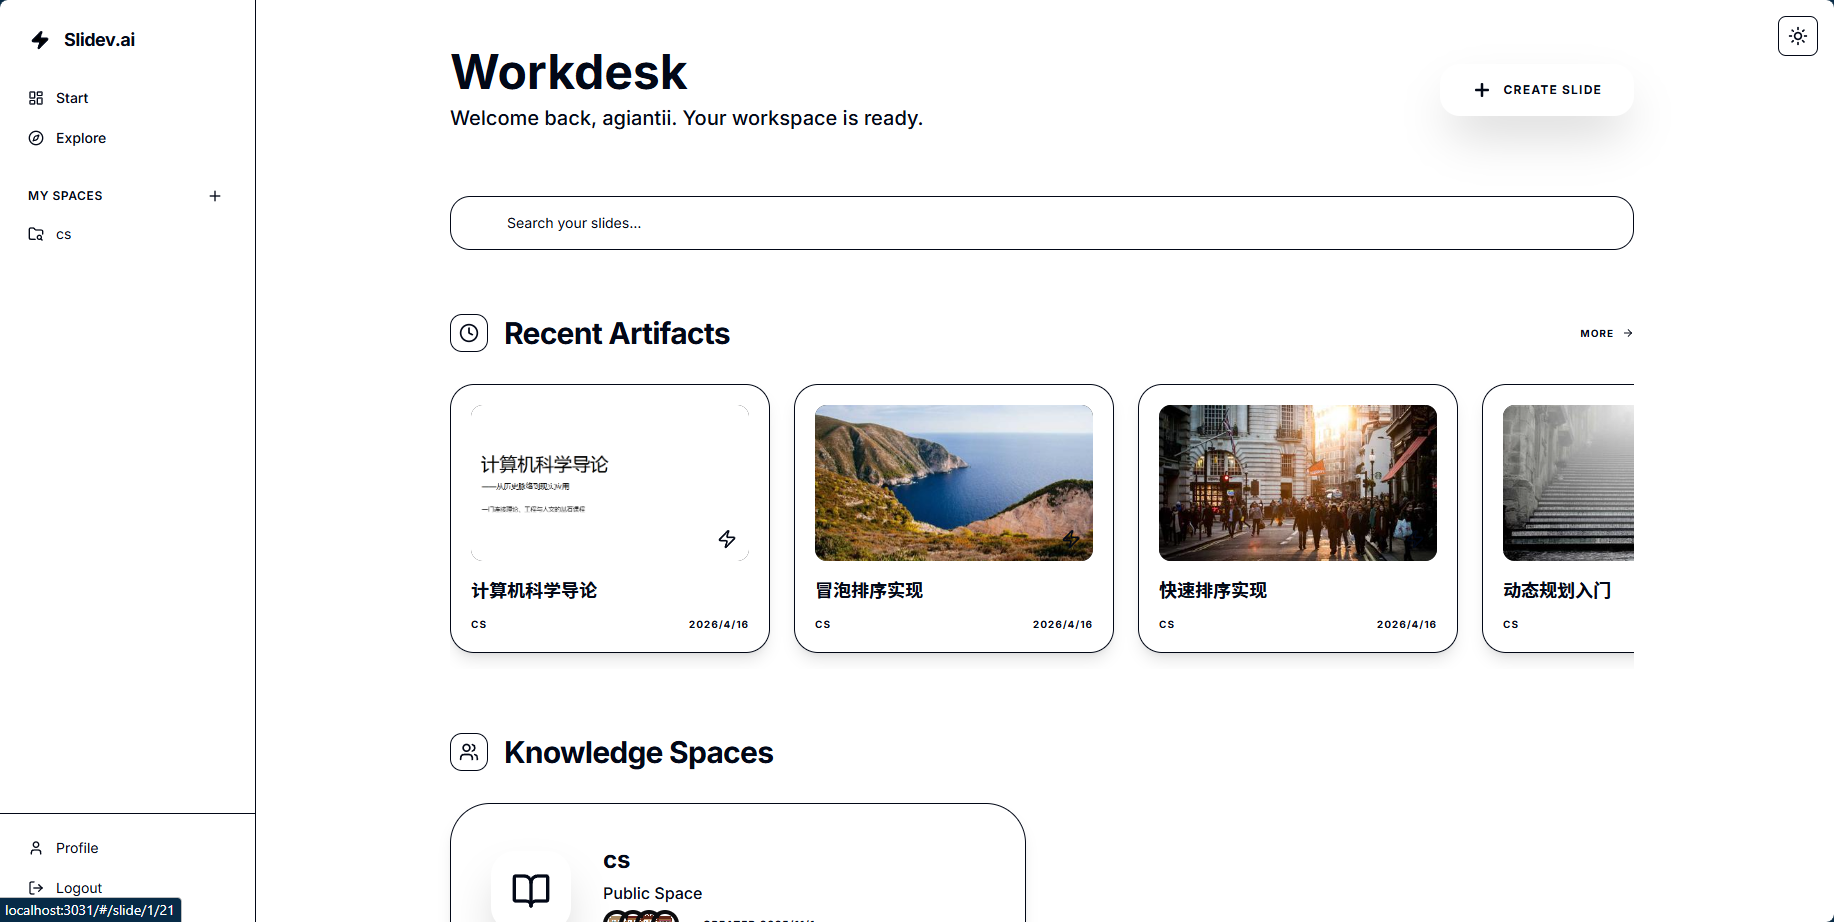
\includegraphics[width=0.9\textwidth]{figures/appt/start.png}
        \caption{智能幻灯片协作平台工作台界面}
        \label{fig:home-interface}
    \end{figure}

    \begin{figure}[htbp]
        \centering
        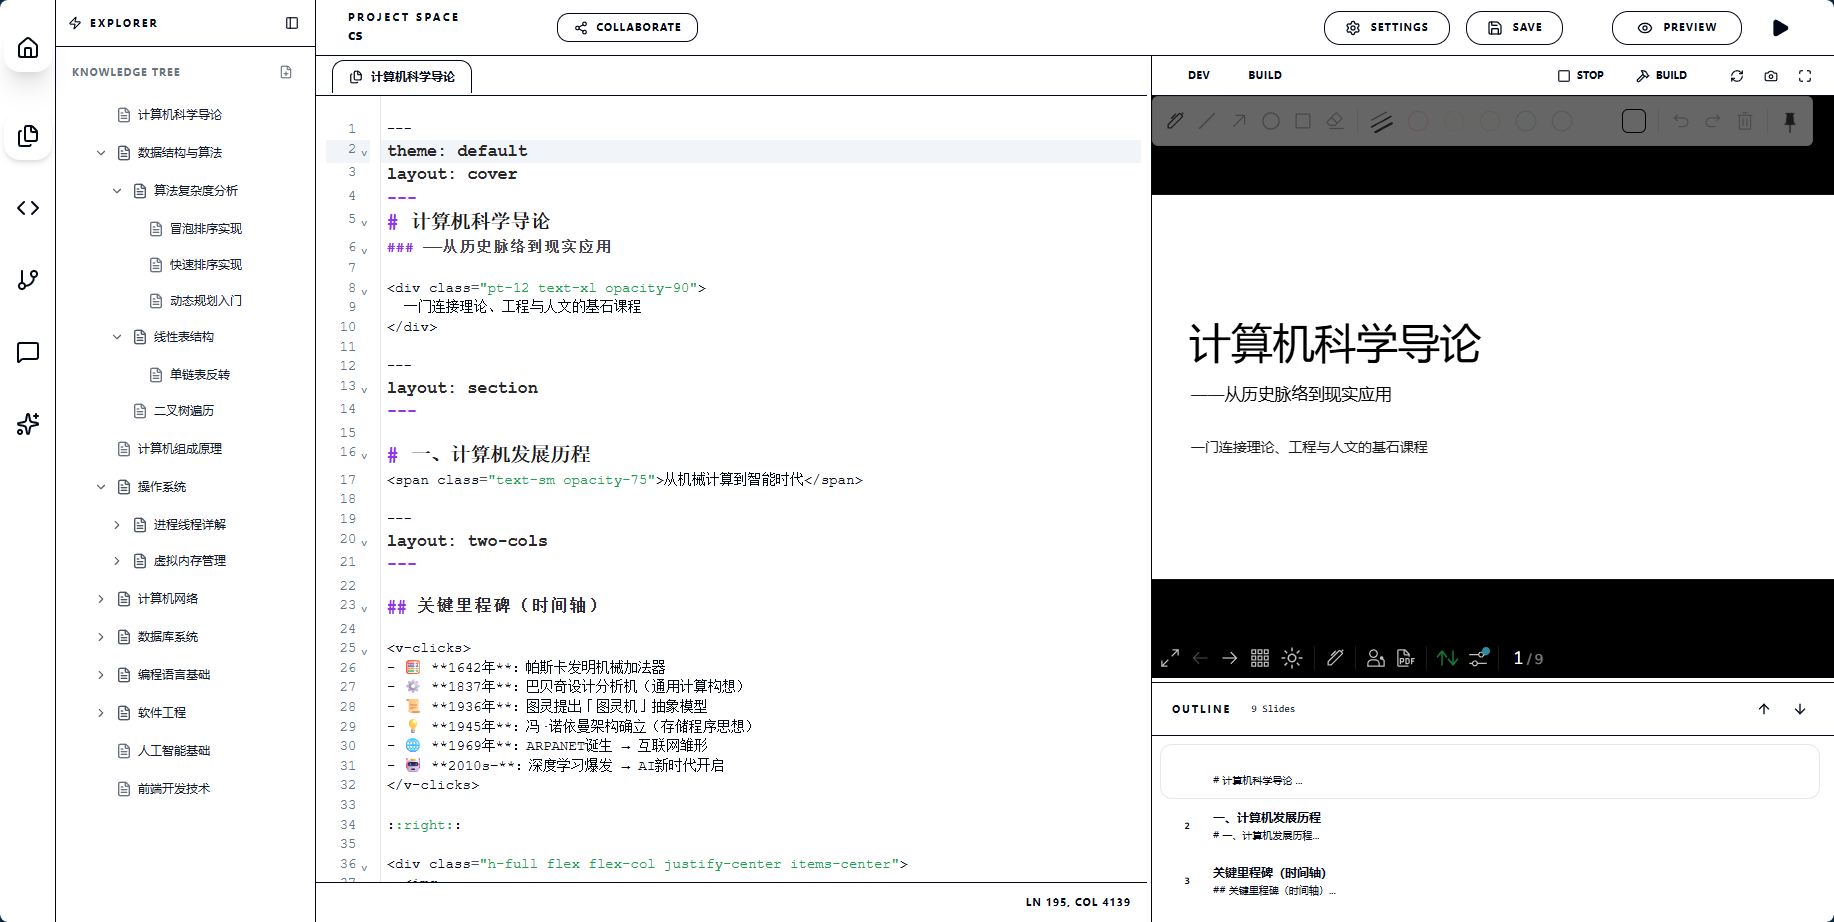
\includegraphics[width=0.9\textwidth]{figures/appt/editor.png}
        \caption{智能幻灯片协作平台编辑器界面}
        \label{fig:editor-interface}
    \end{figure}

    \begin{figure}[htbp]
        \centering
        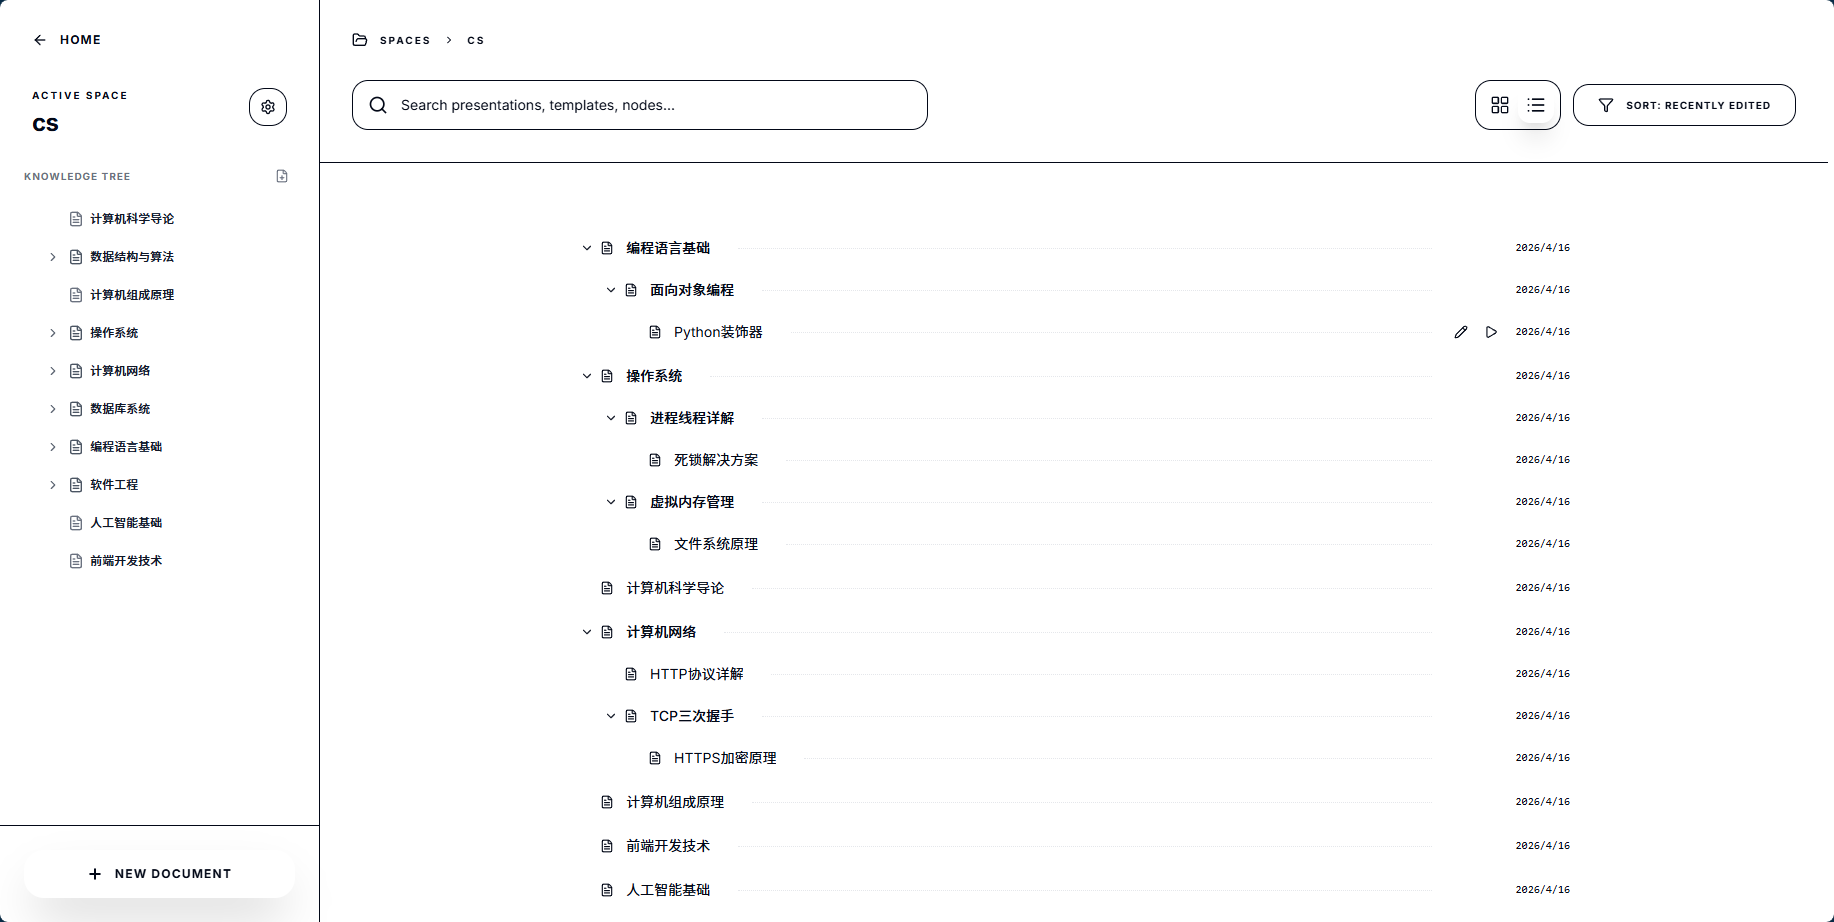
\includegraphics[width=0.9\textwidth]{figures/appt/slideSpace.png}
        \caption{智能幻灯片协作平台幻灯片空间管理界面}
        \label{fig:slideSpace-interface}
    \end{figure}

    \begin{figure}[htbp]
        \centering
        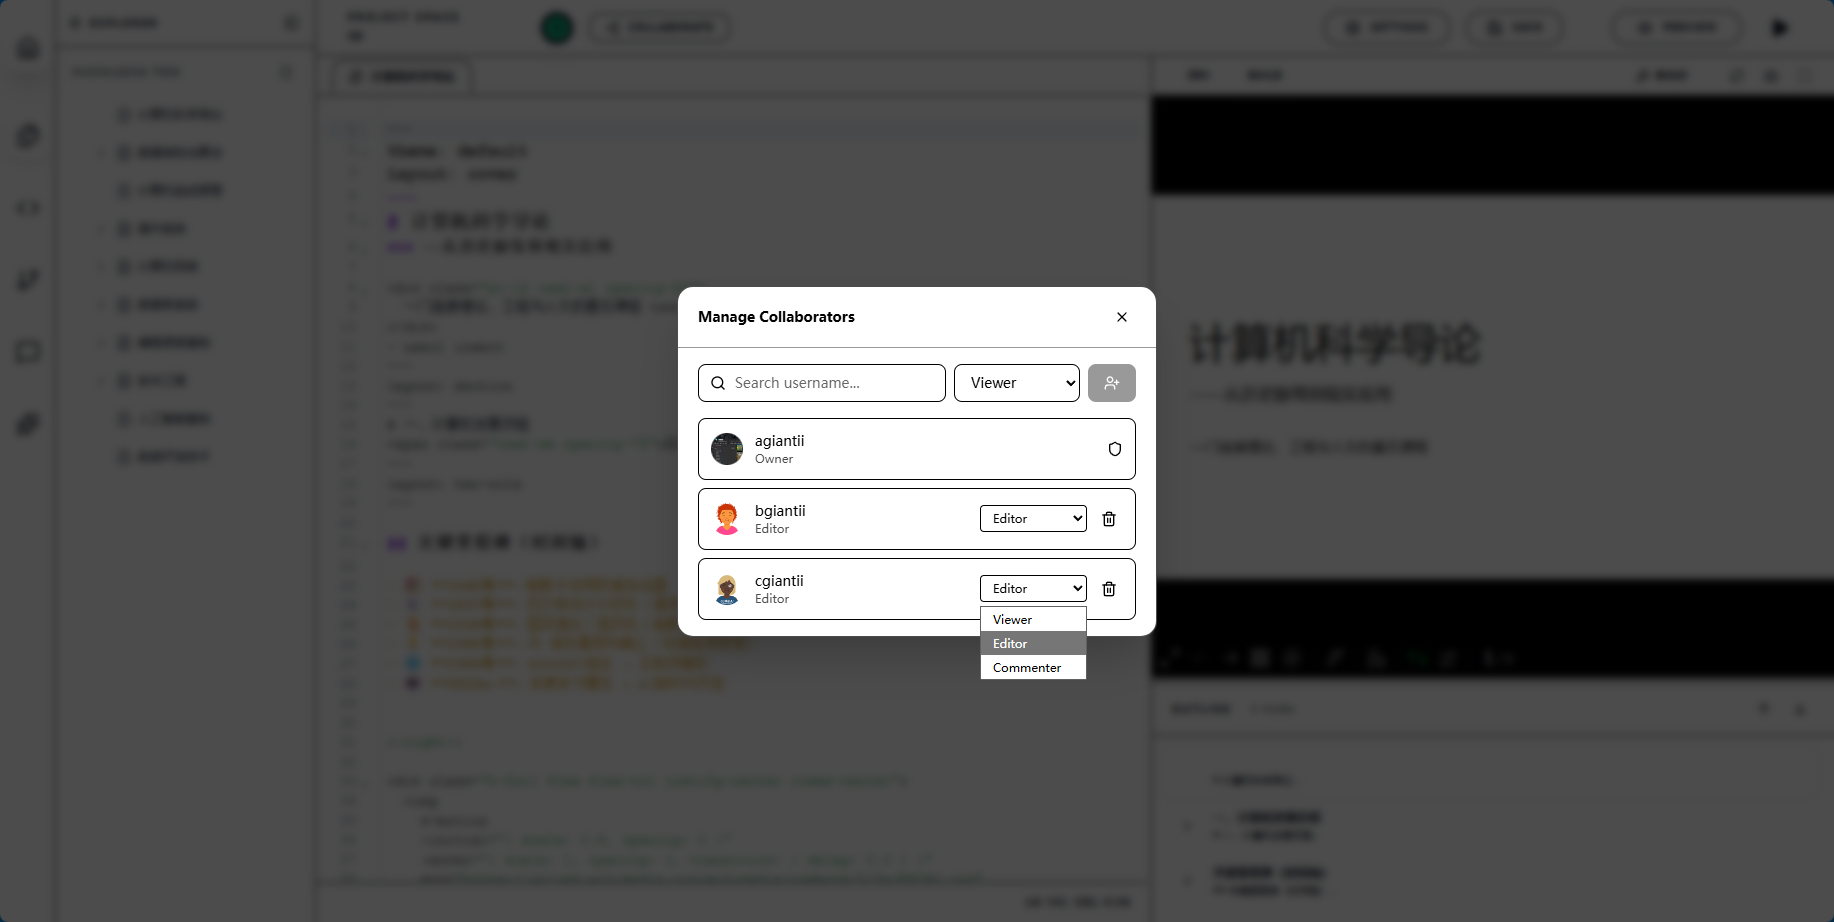
\includegraphics[width=0.9\textwidth]{figures/appt/permission-panel-pure-white.png}
        \caption{智能幻灯片协作平台权限管理面板界面}
        \label{fig:permission-panel-interface}
    \end{figure}

    \section{核心功能使用指南}\label{sec:core-features-guide}

    \subsection{实时协作编辑}

    本平台基于Yjs CRDT算法实现了无冲突的实时协作编辑功能 ，支持多用户同时编辑同一文档,如\ref{fig:shared-doc-presentation-interface}所示：

    \begin{figure}[htbp]
        \centering
        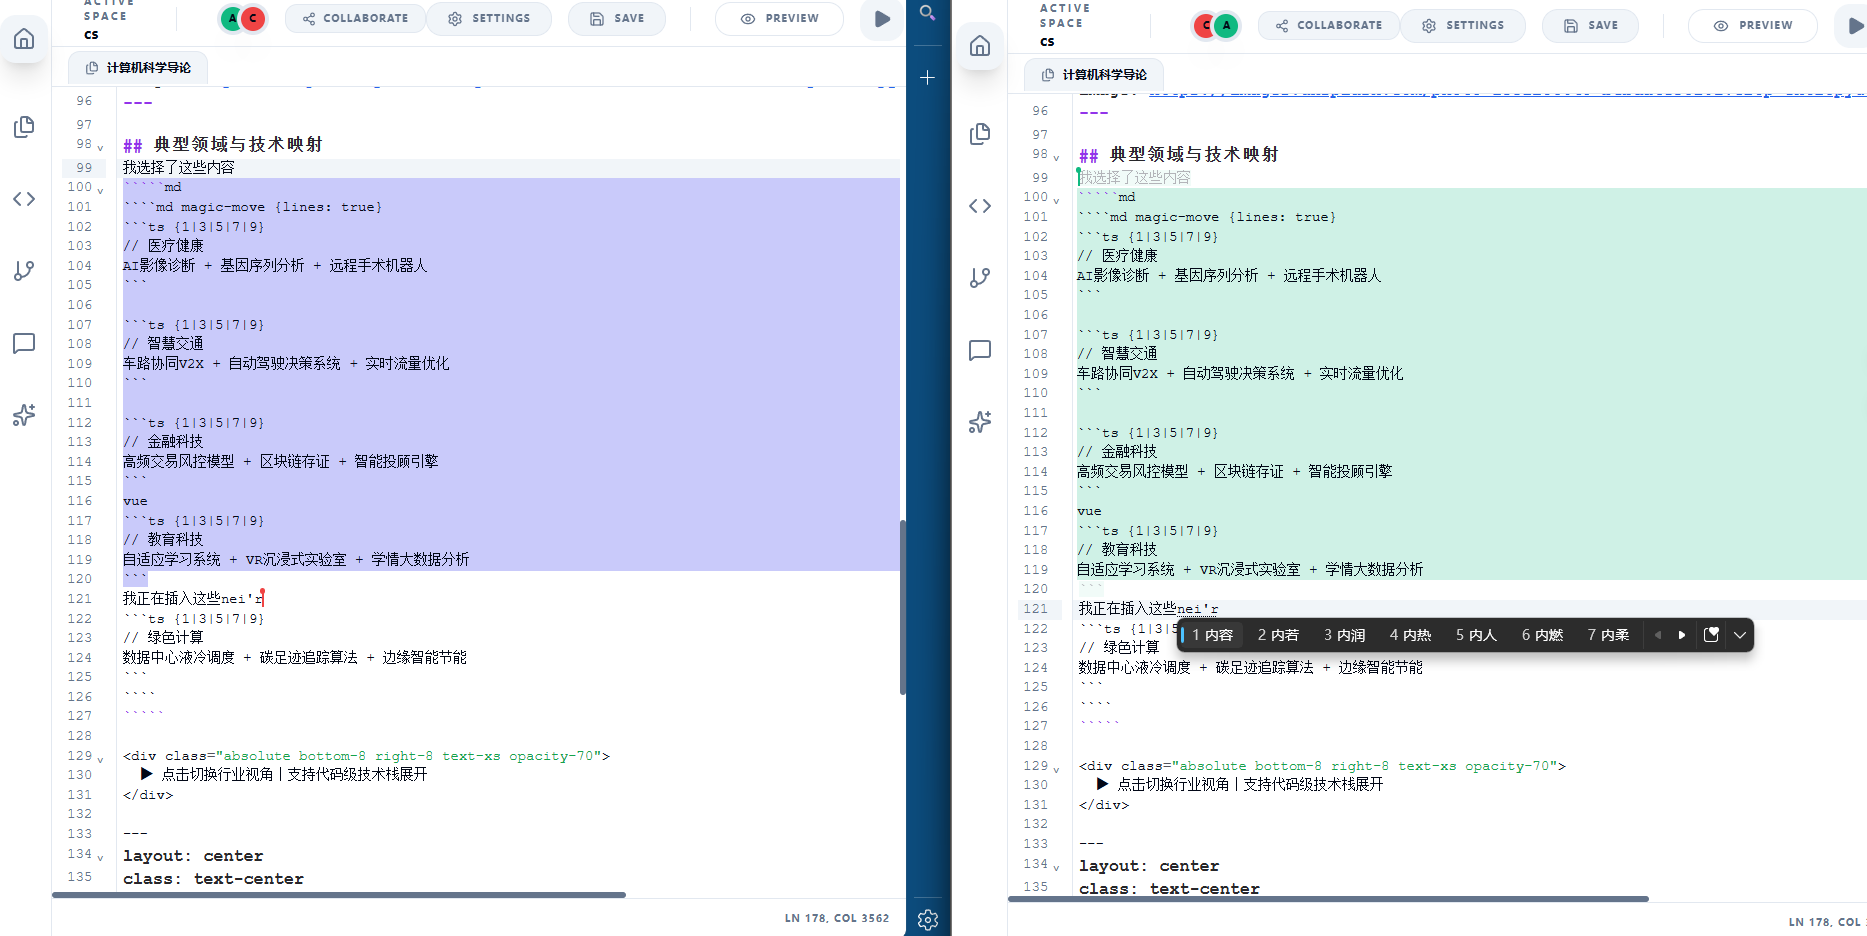
\includegraphics[width=0.95\textwidth]{figures/appt/shared-doc-presentation.png}
        \caption{智能幻灯片协作平台共享文档演示界面}
        \label{fig:shared-doc-presentation-interface}
    \end{figure}
    \textbf{邀请协作者}：在编辑器右上角的协作面板中点击“邀请成员”按钮，输入协作者的用户名并选择角色权限（Owner/Editor/Commenter/Viewer）。\textbf{实时光标追踪}：协作者在编辑文档时，其他用户可以在编辑器中看到其实时光标位置和选中内容，不同用户以不同颜色区分。\textbf{在线状态显示}：协作面板实时显示当前在线的协作者列表，包括头像、用户名和编辑状态。\textbf{协同编辑操作}：多个用户可以同时编辑文档的不同部分，系统自动解决编辑冲突，确保最终一致性。所有编辑操作实时同步到所有在线用户。

    \begin{leftbar}
        \noindent\textbf{使用建议：}实时协作编辑特别适合团队会议、远程协作和共同创作场景。建议在开始协作前明确文档结构和编辑分工，避免多个用户同时修改同一段落造成混淆。
    \end{leftbar}

    \subsection{权限管理系统}

    平台基于RBAC模型设计了四级权限体系，以确保文档的安全访问和合理使用：\textbf{角色权限定义}：\textbf{Owner}：拥有者，具有所有权限，包括删除文档、管理成员、修改权限等；\textbf{Editor}：编辑者，可以查看、编辑文档内容，添加评论，查看版本历史；\textbf{Commenter}：评论者，可以查看文档内容，添加评论，但不能编辑内容；\textbf{Viewer}：查看者，只能查看文档内容和版本历史，不能进行任何修改。\textbf{权限设置方法}：在协作面板中点击用户角色卡片，可以通过开关按钮灵活调整具体权限。平台提供了图形化的权限管理界面，简化了权限配置流程。\textbf{文档可见性控制}：文档支持公开和私有两种可见性设置。公开文档可以被所有用户查看（根据权限），私有文档只有被授权的用户才能访问。

    \subsection{AI辅助创作}

    本平台集成了大语言模型API，能够提供智能内容生成和创作辅助，如图 \ref{fig:ai-assistant-interface} 和图 \ref{fig:ai-generate-interface} 所示：\textbf{AI面板调用}：使用Ctrl+I快捷键或点击编辑器侧边栏的AI图标打开AI辅助面板。AI面板提供内容生成、语法优化和创意建议等功能。\textbf{内容生成功能}：在AI面板中输入需求描述（如“生成一个关于React Hooks的幻灯片大纲”），AI会自动生成符合Slidev语法的Markdown内容。生成的内容可以直接插入到编辑器中。\textbf{语法适配优化}：AI生成的内容会经过语法适配处理，确保符合Slidev幻灯片语法规范，减少用户手动调整的工作量。\textbf{智能建议系统}：基于当前编辑内容和上下文，AI会提供排版建议、设计优化和内容扩展建议，帮助用户提升幻灯片质量。\textbf{图像生成功能}：平台集成AI图像生成能力，可以根据文本描述生成配图，支持技术图表、概念图示和装饰性图片等多种类型。
    
    \begin{leftbar}
        \noindent\textbf{使用建议：}AI辅助功能适合快速生成初稿、获取创意灵感和优化表达方式。建议用户先提供清晰的上下文和具体要求，生成结果后根据需要进行调整和优化。
    \end{leftbar}
    
    \begin{figure}[htbp]
        \centering
        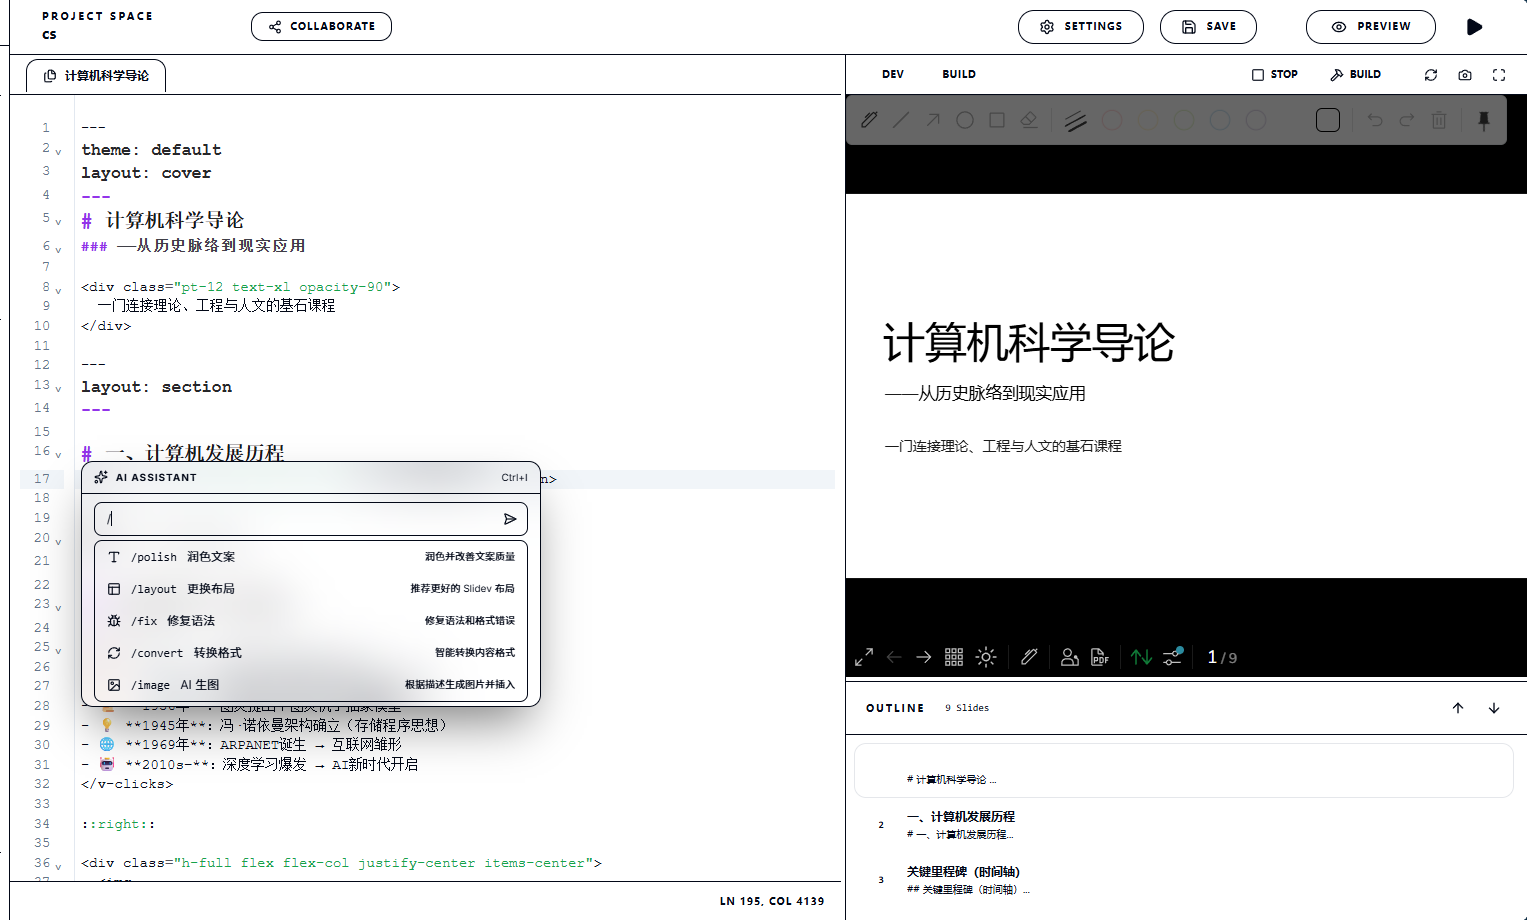
\includegraphics[width=0.9\textwidth]{figures/appt/ai-assistant.png}
        \caption{智能幻灯片协作平台AI辅助功能界面}
        \label{fig:ai-assistant-interface}
    \end{figure}

    \begin{figure}[htbp]
        \centering
        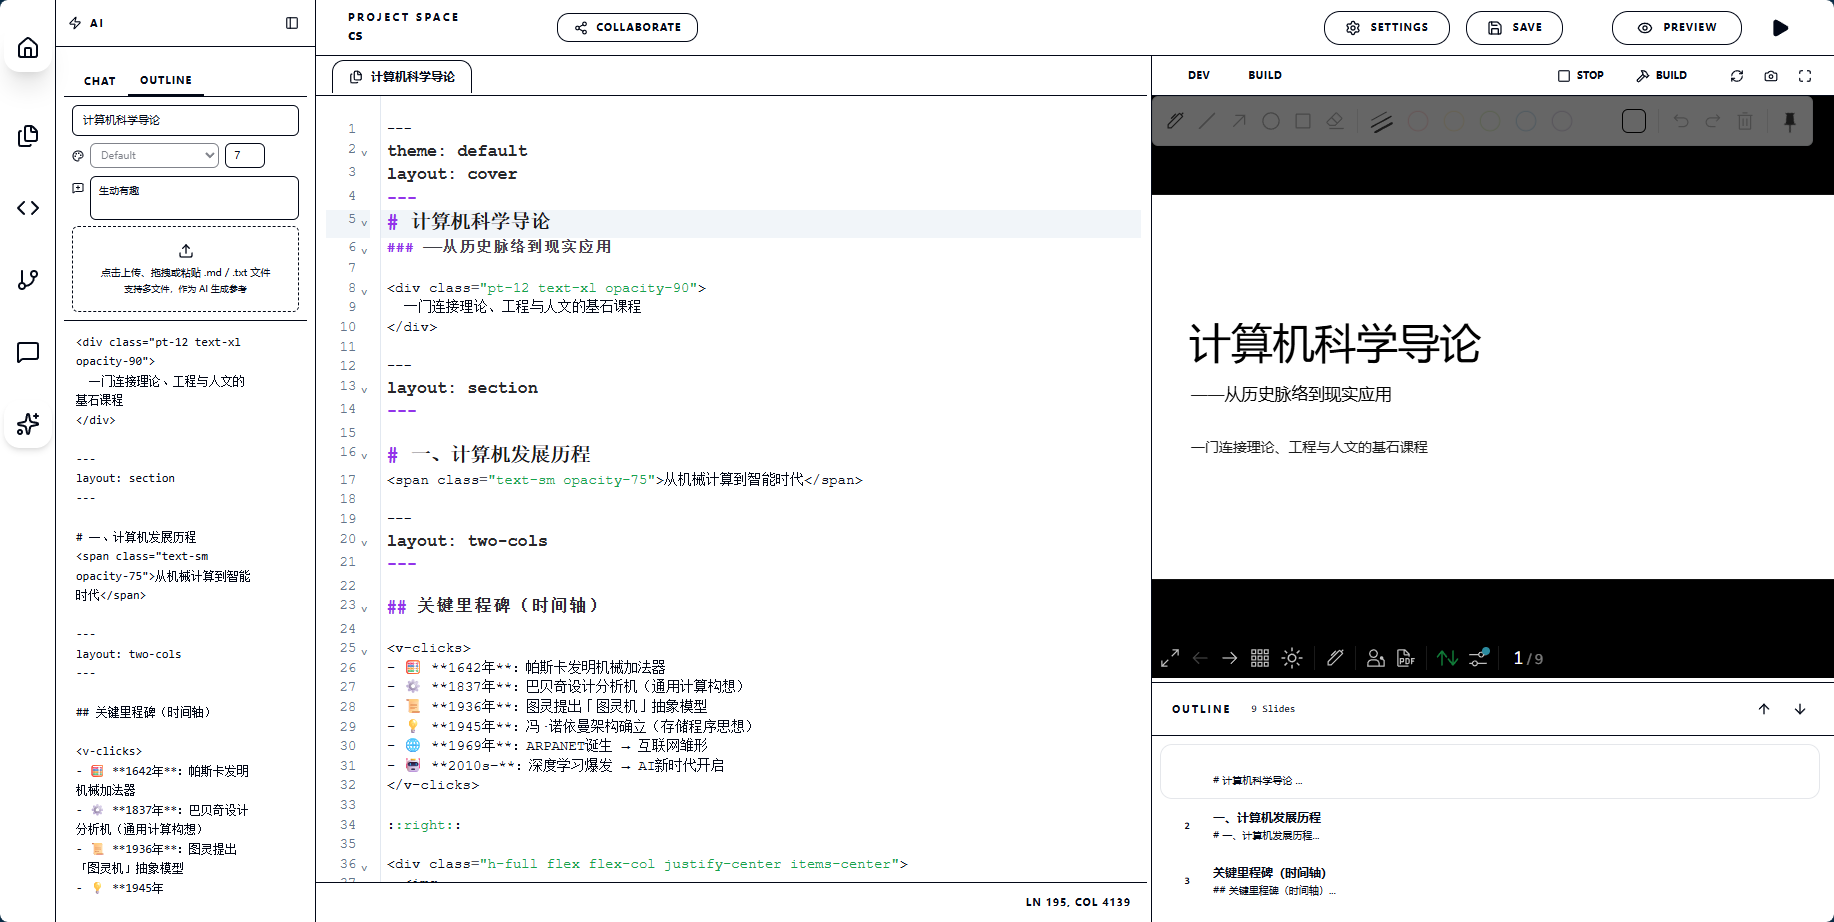
\includegraphics[width=0.9\textwidth]{figures/appt/ai-gernerate.png}
        \caption{智能幻灯片协作平台AI内容生成界面}
        \label{fig:ai-generate-interface}
    \end{figure}


    \subsection{幻灯片编辑基础}

    平台基于CodeMirror 6提供专业的Markdown编辑体验：\textbf{Markdown语法支持}：支持标准的Markdown语法，包括标题、列表、链接、图片、代码块等。幻灯片页面使用`---`分隔符创建。\textbf{实时预览功能}：右侧预览窗口提供Dev/Build双模式预览。Dev模式实时显示编辑效果，Build模式展示最终渲染效果。\textbf{语法高亮}：编辑器支持多种编程语言的语法高亮，包括JavaScript、TypeScript、Python、Java等，适合技术演示场景。\textbf{大纲导航}：左侧大纲面板显示文档结构，点击大纲节点可以快速定位到对应内容，编辑器与预览窗口同步滚动。\textbf{快捷键操作}：Ctrl+S：保存当前文档；Ctrl+Shift+S：创建新版本；Ctrl+B：显示/隐藏左侧菜单；Ctrl+Alt+B：显示/隐藏右侧预览；Ctrl+I：显示/隐藏AI面板；Ctrl+V：插入图片（自动上传到OSS）。

    \section{高级功能详解}\label{sec:advanced-features}

    \subsection{版本控制系统}

    平台提供简化的版本控制功能，降低Git等专业工具的使用门槛，如图 \ref{fig:version-control-interface} 所示：\textbf{自动保存机制}：系统定期自动保存文档内容，防止数据丢失。用户也可以使用Ctrl+S快捷键手动保存。\textbf{手动版本创建}：使用Ctrl+Shift+S快捷键或点击版本控制面板中的“创建版本”按钮，可以手动创建重要版本并添加提交消息说明。\textbf{版本历史查看}：在版本控制面板中查看文档的所有历史版本，包括版本号、创建时间、创建者和提交消息。\textbf{差异对比功能}：选择两个版本进行差异对比，系统以可视化方式显示内容变化，包括添加、删除和修改的部分。\textbf{一键回滚操作}：选择任意历史版本，点击“回滚到此版本”按钮可以将文档内容恢复到指定版本状态。回滚操作会创建新的版本记录，不影响历史版本数据。

    \begin{figure}[htbp]
        \centering
        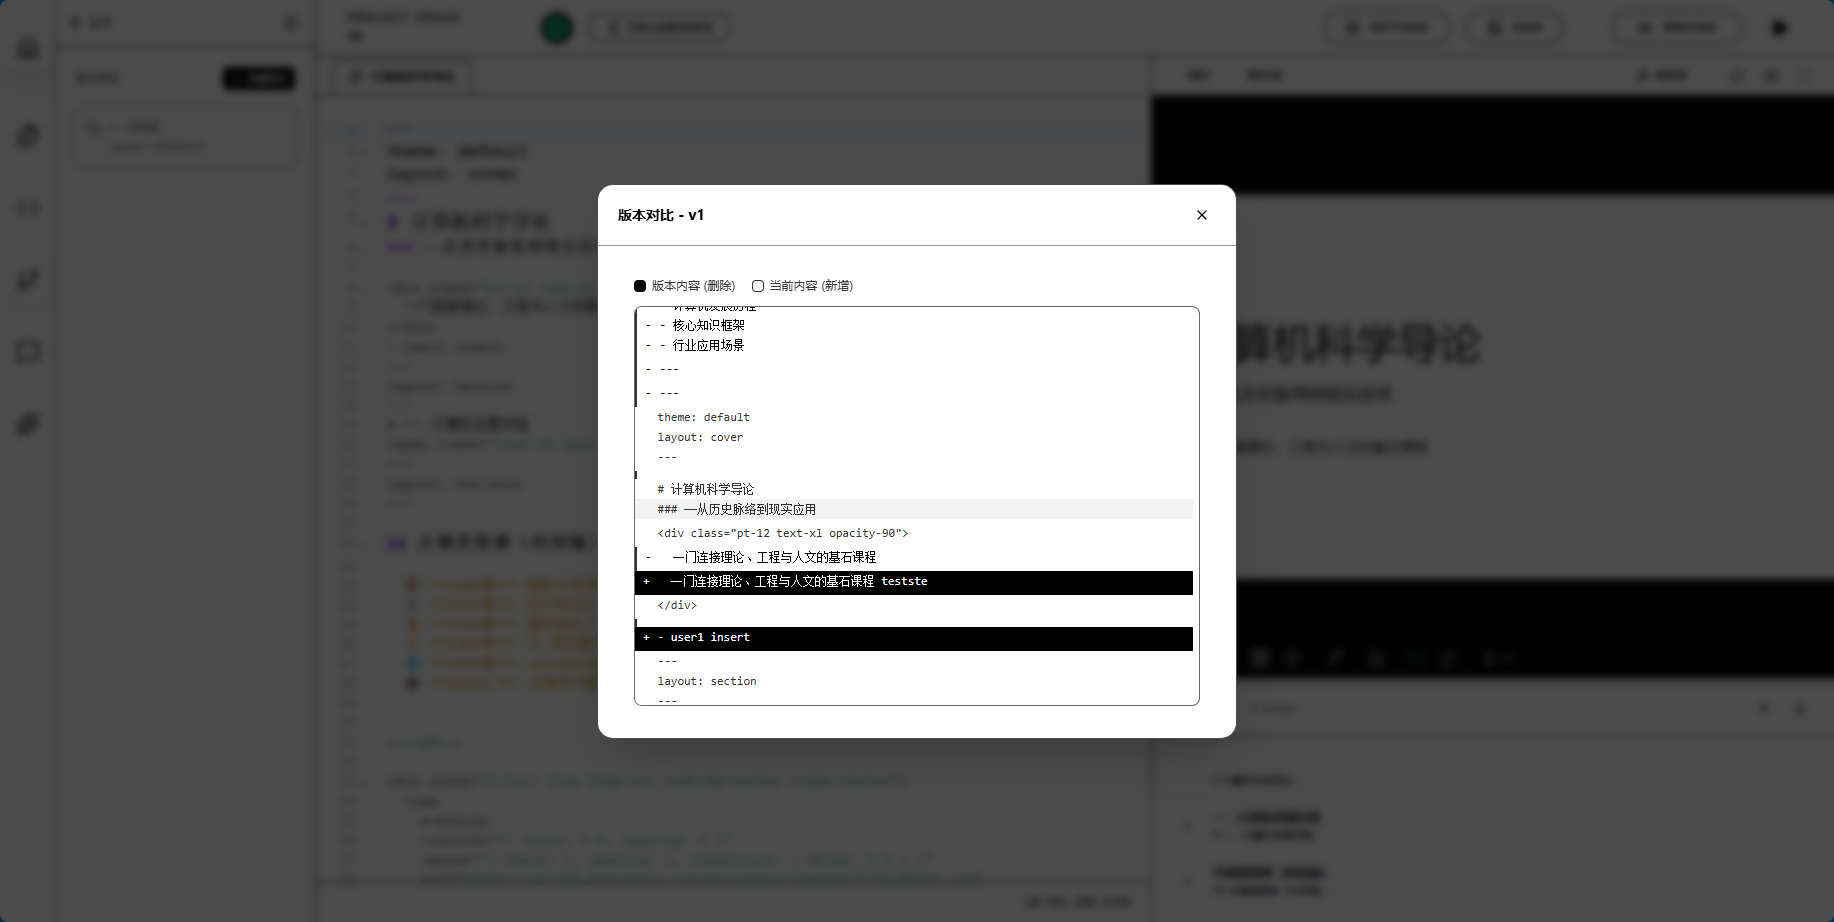
\includegraphics[width=0.9\textwidth]{figures/appt/version-control-wh&bl.png}
        \caption{智能幻灯片协作平台版本控制界面}
        \label{fig:version-control-interface}
    \end{figure}

    % \begin{figure}[htbp]
    %     \centering
    %     \begin{tikzpicture}[
    %         timeline/.style={rectangle, draw, fill=blue!5, align=left, minimum width=7.5cm, minimum height=1cm},
    %         diffbox/.style={rectangle, draw, fill=green!5, align=left, minimum width=7.5cm, minimum height=2.8cm},
    %         button/.style={rectangle, draw, fill=orange!20, rounded corners, align=center, minimum width=1.8cm, minimum height=0.8cm},
    %         arrow/.style={->, >=stealth, thick},
    %         label/.style={font=\small}
    %     ]

    %     % 时间轴区域
    %     \node[timeline] (timeline) at (0, 3.5) {
    %         \textbf{版本历史时间轴}\quad
    %         \begin{tikzpicture}[scale=0.8]
    %             \draw[->] (0,0) -- (6,0);
    %             \foreach \x/\text in {0/初始版本, 1.5/v1.1, 3/v1.2, 4.5/v1.3, 6/当前版本}
    %                 \draw (\x,0.1) -- (\x,-0.1) node[below, label] {\text};
    %             \draw[fill=red] (4.5,0) circle (0.08);
    %             \node[label, above] at (4.5,0.1) {选中};
    %         \end{tikzpicture}
    %     };

    %     % 版本列表
    %     \node[timeline, below=0.8cm of timeline, minimum height=2.5cm] (versionlist) {
    %         \begin{tabular}{llll}
    %             \textbf{版本号} & \textbf{创建时间} & \textbf{创建者} & \textbf{提交消息} \\
    %             v1.3 & 2025-12-28 10:30 & 张三 & 添加AI辅助功能 \\
    %             v1.2 & 2025-12-27 15:20 & 李四 & 修复权限管理bug \\
    %             v1.1 & 2025-12-26 09:15 & 王五 & 优化实时协作性能 \\
    %             v1.0 & 2025-12-25 14:00 & 张三 & 初始版本 \\
    %         \end{tabular}
    %     };

    %     % 差异对比区域
    %     \node[diffbox, below=0.8cm of versionlist] (diff) {
    %         \textbf{差异对比视图}\\
    %         \begin{tikzpicture}[scale=0.9]
    %             \draw[fill=green!20] (0,0) rectangle (7,1.2);
    %             \node[label, anchor=north west] at (0,1.2) {\texttt{+ 添加AI辅助面板功能}};
    %             \node[label, anchor=north west] at (0,0.9) {\texttt{- 移除旧版编辑器代码}};
    %             \node[label, anchor=north west] at (0,0.6) {\texttt{* 优化权限验证逻辑}};
    %             \node[label, anchor=north west] at (0,0.3) {\texttt{+ 新增Slidev主题支持}};
    %         \end{tikzpicture}
    %     };

    %     % 操作按钮
    %     \node[button] (rollback) at (-2, -3.5) {一键回滚};
    %     \node[button] (compare) at (0, -3.5) {对比版本};
    %     \node[button] (create) at (2, -3.5) {创建版本};

    %     % 连接线
    %     \draw[arrow, dashed] (versionlist.south) -- node[right, label] {选择版本} (diff.north);
    %     \draw[arrow] (rollback) -- (-2, -3) -- (diff.south);
    %     \draw[arrow] (compare) -- (0, -3) -- (diff.south);
    %     \draw[arrow] (create) -- (2, -3) -- (diff.south);

    %     % 标签
    %     \node[label, above=0.1cm of timeline] {\textbf{版本历史浏览}};
    %     \node[label, above=0.1cm of diff] {\textbf{内容变化可视化}};
    %     \node[label, below=0.1cm of diff] {\textbf{操作控制区}};

    %     \end{tikzpicture}
    %     \caption{智能幻灯片协作平台版本控制界面示意图}
    %     \label{fig:version-control-ui}
    % \end{figure}

    \subsection{代码片段管理}

    平台提供代码片段管理系统，支持可复用代码块的存储和插入，如图 \ref{fig:snippets-interface} 所示：\textbf{创建代码片段}：在编辑器中选中代码内容，右键选择“保存为代码片段”，输入片段名称和描述信息。代码片段会保存到用户的个人片段库中。\textbf{插入代码片段}：在编辑器中点击插入菜单的“代码片段”选项，从片段库中选择需要的代码片段插入到当前光标位置。支持按名称搜索和按语言分类筛选。\textbf{管理片段库}：在设置页面的代码片段管理界面中，用户可以查看、编辑、删除和分类管理所有个人代码片段。

    \begin{figure}[!htbp]
        \centering
        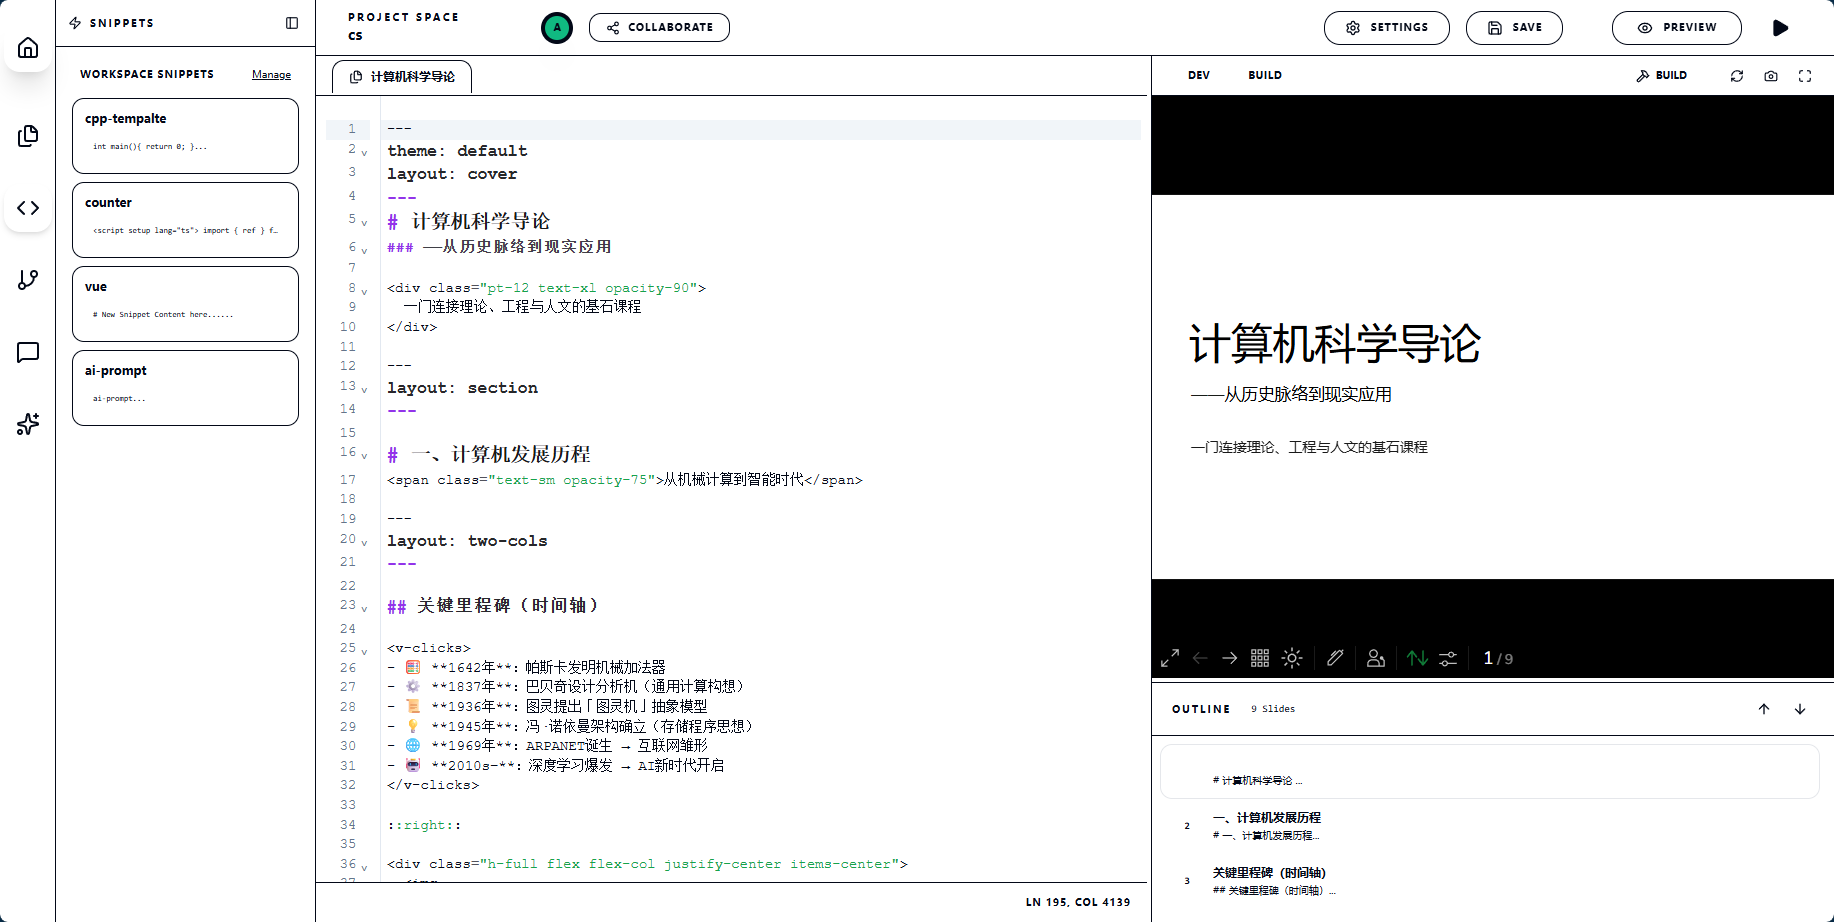
\includegraphics[width=0.95\textwidth]{figures/appt/snippets.png}
        \caption{智能幻灯片协作平台代码片段管理界面}
        \label{fig:snippets-interface}
    \end{figure}

    \subsection{评论与讨论系统}

    平台集成评论功能，支持文档内容的讨论和反馈，如图 \ref{fig:comment-interface} 所示：\textbf{添加评论}：在编辑器中选中文本内容，点击出现的评论图标或使用右键菜单添加评论。评论支持Markdown格式，可以包含代码块和链接。\textbf{回复评论}：在现有评论下方可以添加回复，形成讨论线程。评论系统支持树形结构，便于跟踪讨论脉络。

    \begin{figure}[htbp]
        \centering
        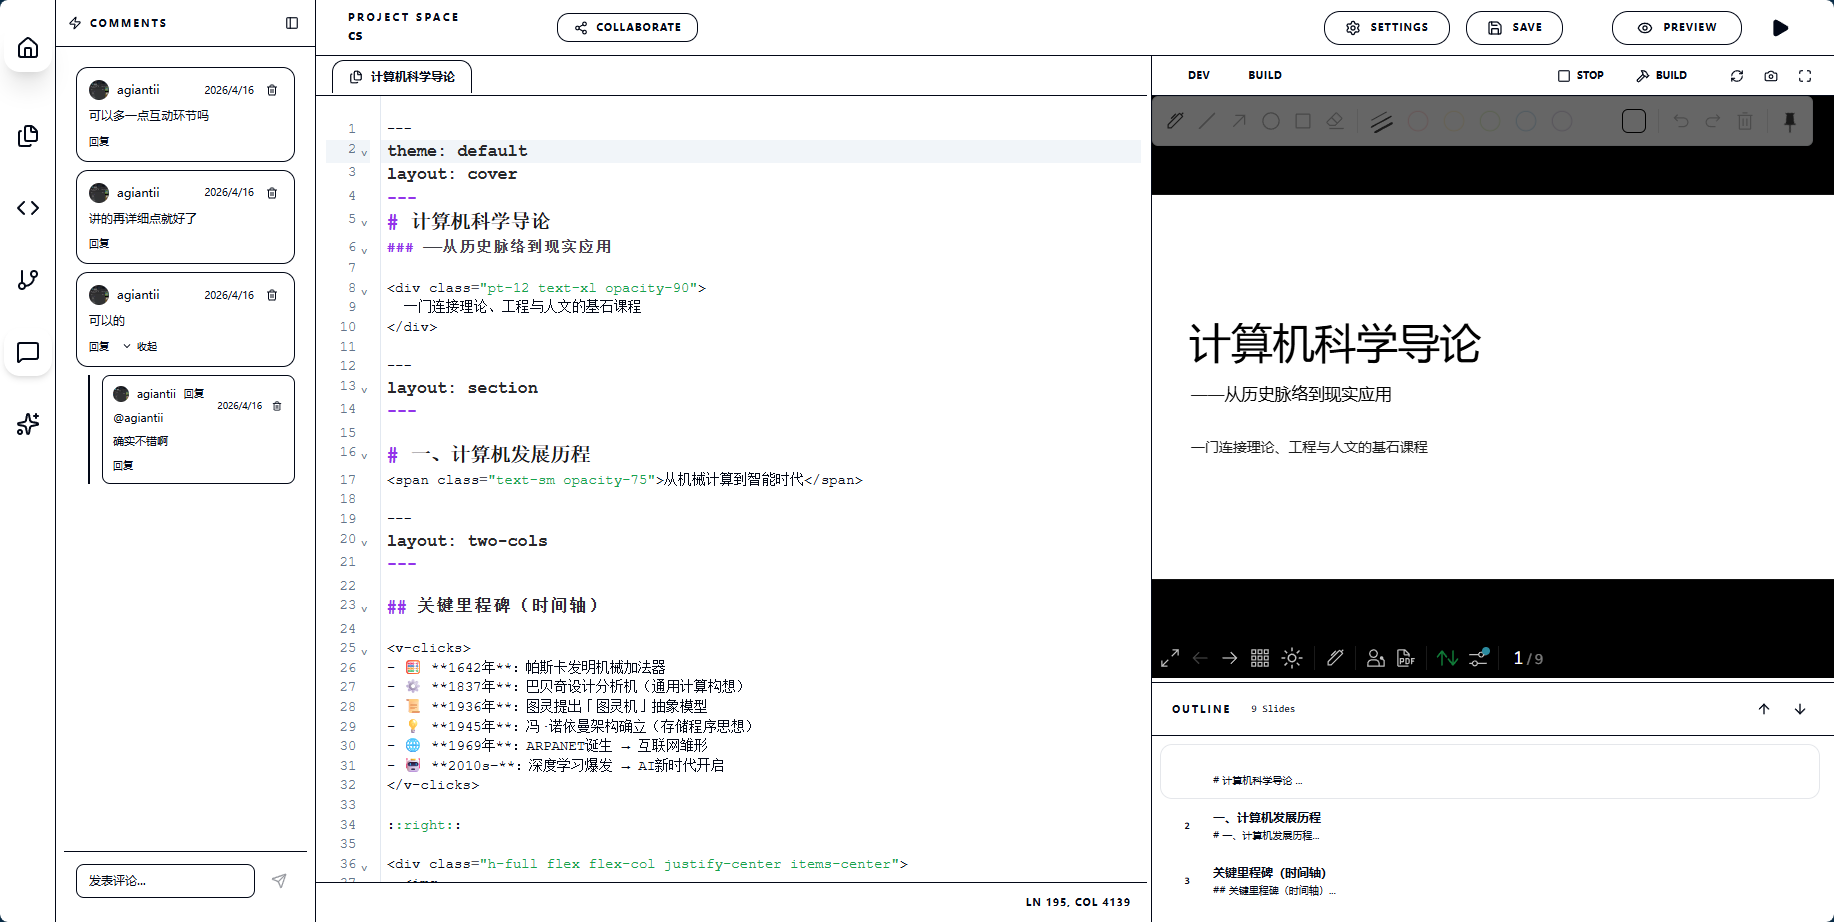
\includegraphics[width=0.95\textwidth]{figures/appt/comment.png}
        \caption{智能幻灯片协作平台评论系统界面}
        \label{fig:comment-interface}
    \end{figure}

    \subsection{幻灯片空间管理}

    幻灯片空间是组织和管理幻灯片文档的知识库系统：\textbf{创建空间}：在工作台界面点击“创建空间”按钮，输入空间名称、描述和可见性设置。\textbf{文档组织}：空间支持文档的树形结构组织，可以通过拖拽调整文档顺序和层级关系。文档支持父子关系，便于构建知识体系。\textbf{全局搜索}：平台提供全局搜索功能，可以跨空间搜索文档标题和内容，快速定位目标文档。

    \subsection{主题与插件系统}

    平台支持Slidev主题和插件，提供丰富的视觉效果和功能扩展：\textbf{主题选择}：在编辑器设置中选择不同的Slidev主题，改变幻灯片的整体视觉效果。平台内置多种专业主题，支持浅色和深色模式。\textbf{插件管理}：Slidev插件提供额外功能，如数学公式渲染、图表绘制、动画效果等。平台内置常用插件，支持插件启用/禁用管理。\textbf{插件开发}：平台提供插件开发接口，开发者可以基于Slidev插件规范开发自定义功能插件，扩展平台能力。

    \section{最佳实践与技巧}\label{sec:best-practices}

    \subsection{团队协作流程建议}

    基于本平台的团队协作最佳实践：\textbf{明确角色分工}：根据团队成员的专业领域和职责分配适当的文档权限。建议设立文档负责人（Owner）负责最终审核和发布。\textbf{建立协作规范}：制定团队协作规范，包括文档结构标准、命名规则、评论使用规范等，提高协作效率。\textbf{版本管理策略}：重要里程碑或重大修改时创建手动版本并添加详细的提交消息，便于版本追溯和内容回滚。\textbf{定期同步会议}：建议定期举行文档同步会议，利用平台的实时协作功能进行集体编辑和讨论，提高决策效率。\textbf{知识库维护}：利用幻灯片空间构建团队知识库，按项目或主题组织文档，促进知识积累和共享。

    \subsection{效率提升技巧}

    提高本平台使用效率的技巧和建议：\textbf{快捷键熟练使用}：熟练掌握常用快捷键（如Ctrl+S、Ctrl+B、Ctrl+I等），减少鼠标操作，提高编辑效率。\textbf{代码片段重用}：将常用的代码示例、配置模板保存为代码片段，避免重复输入，保证代码准确性。\textbf{AI辅助优化}：利用AI生成初稿和获取建议，重点关注内容创意和结构优化，提高创作效率。\textbf{模板化创作}：为不同类型的幻灯片创建模板（如技术分享、项目汇报、教学课件），保持团队输出的一致性。\textbf{评论有效使用}：使用评论功能进行异步讨论和反馈，减少会议时间，提高沟通效率。

    \subsection{常见问题解决方案}

    平台使用过程中常见问题的解决方法：\textbf{编辑冲突问题}：当多个用户同时编辑同一段落时，系统会自动解决冲突。如有疑问，可以通过版本历史查看具体修改内容。\textbf{权限访问问题}：如果无法访问文档或执行某些操作，检查自己的角色权限。联系文档所有者或管理员调整权限设置。\textbf{图片上传失败}：检查网络连接和图片格式（支持PNG、JPG、GIF等常见格式）。图片大小建议不超过5MB。\textbf{AI生成不准确}：提供更详细的上下文和具体要求，重新生成内容。也可以手动调整AI生成的内容以满足需求。\textbf{版本回滚恢复}：如果不慎回滚到错误版本，可以从版本历史中选择正确的版本再次回滚。所有版本记录都会保留。\textbf{浏览器兼容问题}：建议使用最新版本的Chrome、Firefox、Edge或Safari浏览器。清除浏览器缓存可以解决部分显示问题。

    \subsection{高级功能进阶使用}

    进阶用户的高级功能使用建议：\textbf{API集成开发}：平台提供RESTful API接口，支持与第三方系统集成。可以开发自动化脚本进行批量文档处理。\textbf{自定义主题开发}：基于Slidev主题规范开发定制主题，满足特定视觉品牌需求。主题开发需要CSS和Vue.js基础知识。\textbf{协作流程自动化}：利用Webhook和API接口实现协作流程自动化，如文档状态变更通知、权限自动调整等。\textbf{数据导出与分析}：平台支持文档内容导出为Markdown、PDF等格式。可以通过API获取使用数据进行分析和统计。\textbf{企业级部署优化}：对于企业用户，可以考虑私有化部署方案，配置自定义域名、SSL证书和企业用户管理系统。

    \section{总结}\label{sec:guide-summary}

    本章详细介绍了本平台的使用指南，涵盖了平台概述、核心功能使用、高级功能详解和最佳实践等内容。通过本章的学习，用户可以：了解本平台的基本概念和功能特点，掌握快速入门方法。运用最佳实践和技巧，优化工作流程，提升幻灯片创作质量和效率。

    本平台作为AI驱动的幻灯片协作编辑平台，不仅提供了强大的技术功能，还注重用户体验和协作效率。平台的设计理念是通过技术手段降低使用门槛，让用户能够专注于内容创作和团队协作，而非技术细节。

    随着平台的不断发展和完善，将会提供更多创新的功能和优化的用户体验。用户可以通过平台帮助文档、社区论坛和客户支持获取最新的使用信息和问题解决方案。我们鼓励用户积极反馈使用体验，共同推动平台的改进和发展，使本平台成为更加强大和易用的幻灯片协作工具。

\end{cuzchapter}